\documentclass[a4paper]{article}
\usepackage{vub}

\usepackage{pgfplots}
\usepackage{hyperref}
\usepackage[font=small,labelfont=bf]{caption}
% Some highly suggested packages, please read their manuals.
\usepackage{cleveref}
\usepackage[final]{pdfpages}
\usepackage[square, numbers]{natbib}
\usepackage{float}
\bibliographystyle{abbrvnat}

\newcommand{\dquote}[1]{``#1''}
\newcommand{\squote}[1]{`#1'}
\newcommand{\codes}[1]{\texttt{#1}}


\setlength{\parskip}{\baselineskip}%
\setlength{\parindent}{0pt}%

\title{Project Erlang}
\author{Silken Heynderickx}
\faculty{Science and Bio-Engineering Sciences}
\promotors{Prof. Dr. ???}
\pretitle{Multicore Report (task Erlang) submitted in partial fulfilment of the requirements for the degree of Bachelor of Science in de Computerwetenschappen}
\date{2023-2024}
\pgfplotsset{compat=1.18}

\begin{document}
\maketitle

\tableofcontents

\newpage

\section{Overview}

Briefly summarize your overall implementation approach and the experiments you per-
formed. (1 or 2 paragraphs)

My first implementation was based on users their first character of their username, to put them in a server that has their initial (based on ANSII order). I didn't use this implementation, because first of all when their was a new user added and the dictionary had more users then the treshold, the range of ansii characters was splitted in 2 and the users where moved to the other server. This means that when a user did a new request but was replaced, we needed to keep track of the replaced users to send them their new server, so every request would need to be used to send to the correct server. This is not that big of a problem. Second of all, it is possible that when the range of ANSII characters is splitted in 2, that most to all usernames still fall under the same new range, which causes that the new server is empty and the old one still full. Third, you had to then update all existing servers to update where the users where placed or that servers need to go off (depending on where splitting happend) to find the newly created server. This would cause to have a chain of requests to different servers. Nothing unsolvable, but there were easier and more performant ways to make this implementation working. 
(This implementation is saved under server\_parallelized.erl) 

The implementation I used for the experiments, is based on one server that makes other servers where users can send request too. When a user is registered, it wel get new a server assigned. This doesn't cause a bottleneck because it only handles register requests, or somethimes redirecting requests to another server (ex. when follow user is called). That server holds an ordered dictionary of the usernames with their server saved. Whenever a server is full (depending on threshold), their is a new server created to save new users. Each server has their own users, with their data. When a certain user sends a message, the followers will get that message saved in their timeline (this causes data to be saved on multiple servers). I choose to use here a more performant solution for timeline instead of lower memory usage. When a user follows a new user, the server of the following user wil be saved into the server that requested the PID. So PID will also be saved in different places at the same time, but this has the advantage that the initial server won't have a "too much" of a bottleneck. 

EXPIRMENTS:

\section{Implementation}

\subsection{Architecture}

Describe your project's software architecture on a high level. Use figures to show
how data is distributed over several processes, and how messages flow between them.

\begin{figure}[H]
	\centering
	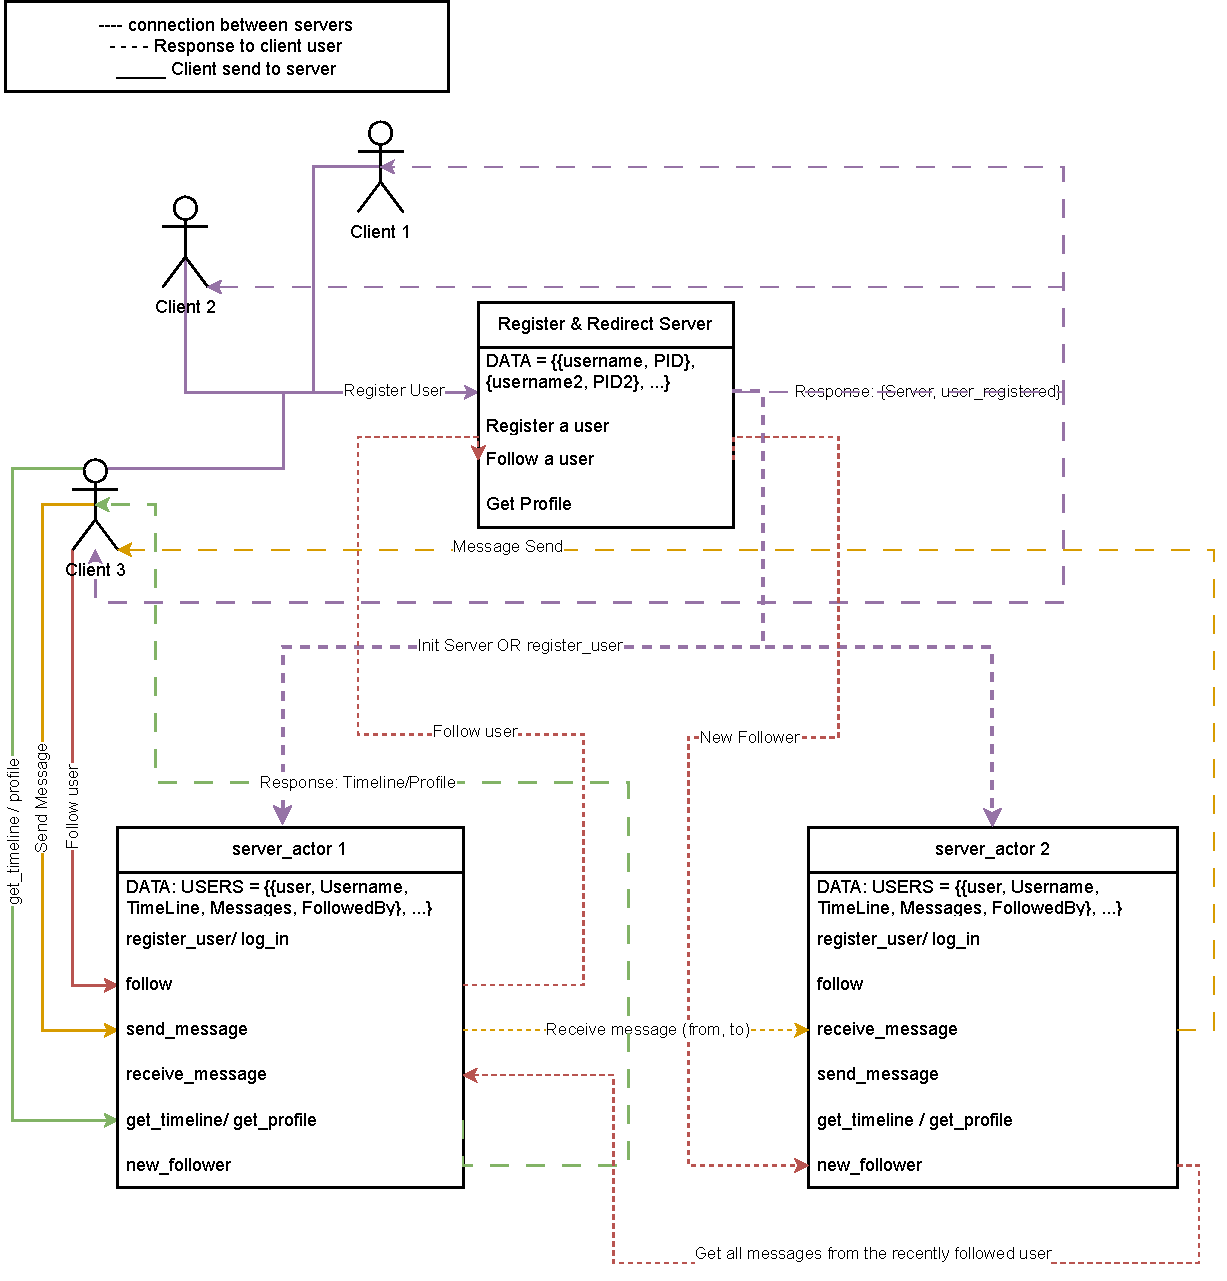
\includegraphics[width = \linewidth]{Architecture.pdf}
	\caption{
		This flowchart gives an overview of the architecture, how messages flow between the actors, and where which data is stored. (Every color of the lines, are new requests from the client and the path it follows)
	}
\end{figure}

For the case of showing the architecture I made 3 clients, these all send Register User to the ''Register \& Redirect Server'', this add the user to an existing server\_actor or makes a new server\_actor depending on the treshold (amount of users per actor).
It sends then the \{PID, user\_registered\} back to the client. When the client receives this message it can send new request tot that server. 

With Client 3, I wanted to display 4 different requests a user can send: "get\_timeline, get\_profile, send\_message, follow".
Get\_timeline and get\_profile, in this case the user asks its own timeline and profile, this is both saved in the actor where the user sends to.
So he will directly send a response back to the user.
In the case that the user is not part of the current actor, it will send do the "Register \& Redirect" to than redirect the message to the correct actor.
This can cause a possible bottleneck when havind lots of register/ follow and get\_profile requests.
This can be solved by saving the actor ID of users in every server\_actor, but when having lots of users, this would cause a many data duplication.
I choose to have data dublication to save the messages, instead of user\_pids.
Because from my experience, when we scroll only we mostly look at the timeline and maybe view a few other profiles.
So I choose to make "get\_timeline" as performant as possible. 

When a user sends a new message, it will send the message to every follower of that user, and save it in their timeline. (What we also could have done here to avoid data dublication but keeping the timeline as performant as possible, is only saving the X most recent messages, and when a users scrolls further than those that the sever will need to go fetch them. But this was out of the scope of this project, because we could not now when a user would looked at all of them.) When getting new messages, they were inserted in an orddict that was already sorted from new to old, so we don't need a sorting algorithm when get\_timeline is called.

When a user follows an other user, the PID will be requested to the Register \& Redirect server, and will to follower will also be send to the followed user. 
Requested the PID of the following user will not cause a dead lock because the server\_actor doesn't wait for a response, but just saves the pid by the correct follower. This can cause some inconsistency in the data of the follower, but often when scrolling online, the timeline doens't get refreshed everytime you follow a new user, so this wil not cause a bit issue. 

% TODO: Implement that a user can also ask the profile from a different user 

%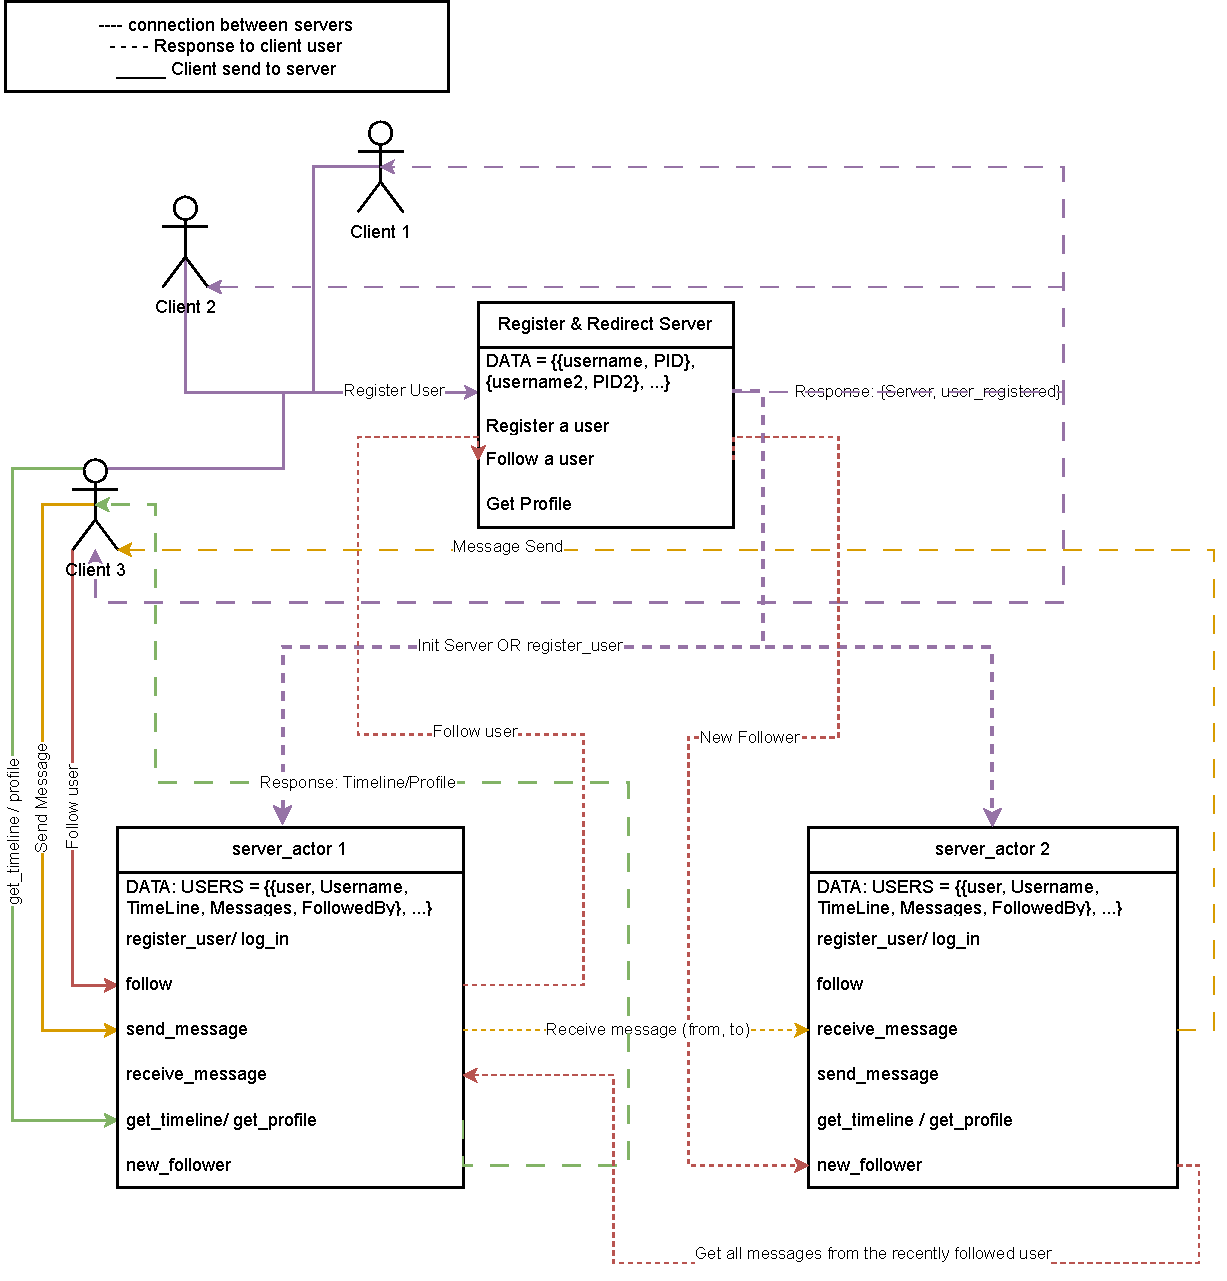
\includepdf[pages=-]{Architecture.pdf}

\subsection{Scalability}

\subsubsection{How does your design ensure scalability? What is the best case and the worst case in
terms of the mix of different user requests? When would the responsiveness decrease?}
The best case of my implementation would be when the requests are mix of request, with a preference to timeline requests and send messages, this would normally not cause any responsiveness decrease. But when there is an overload of register\_user, follow and get\_profile request, the Register and redirect server would get a bottleneck. I focussed on the timeline to be as performant as possible as explained before. I real life this is the most send request, every time you open an app this request will automaticcaly be send.

In most cases, there will not be a chain of register\_user, get\_profile. Sometimes there are follow bots made for users to farm followers, this would cause a big issue for our responsiveness of app. 

\subsubsection{How do you ensure conceptual scalability to hundreds, thousands, or millions of users?
Are there any conceptual bottlenecks left?}

When you choose how much users will be handled per actor, the application is very scalabel. Because of the benchmarks I tried on my local computer, I could conclude that 1 user/ server performs the best, when there are 100 to 1000 users. But when we have an app, ofcource we want that are app is an succes with a goal on those millions of users. When there are millions of user, the changes are very big that the Register and redirect form a bottleneck to the system. This could be resolved by splitting that server in multiple server, that handle different request or handle the requests of users depending on which server they need to contact. But when we talk about million of users the server could also be distributed over the whole world, so the users could send to a server depending on their location. In reality when we talk about millions of users we will not only use parallelism but also distributed systems, which would give us more possiblities to work with.

\subsubsection{ Where did you sacrifice data consistency to improve scalability? How does this decision improve scalability? In which case would the overall data consistency suffer most? }
When you follow a new user and than ask for the timeline, their is a possiblity that the user doesn't know yet which server to connect for the messages of the new follower. This would not cause a big issue, becuase your timeline mostly doesn't refresh when you follow a new user. This improves scalability becuase the server doesn't need to wait for the ID of the server of the follower, so new request can already be send to the server. 

\section{Evaluation}
\subsection{Experimental set-up}
\subsubsection{Which CPU, tools, platform, versions of software, etc. you used }
\textbf{Firefly} \\
CPU: AMD Ryzen Threadripper 3990X Processor (64 core / 128 Threads, at 2.9 GHz base, 4.3 GHz boost) \\
RAM: 12 GB (DDR4 3200 MHz) \\
OS: Ubuntu 20.04.5 (Linux kernel 5.4.0-137-generic) \\
Erlang/OTP version: 22.2.7 \\

\textbf{Local PC:} \\
CPU: 10 cores (6 performance, 4 efficientie) Apple M2 Pro \\
RAM: 16 GB (LPDDR5 Hynix) \\
OS: macOS 14.2.1 (macOS Sonoma) \\
Erlang/OTP version: 26.2.3 \\

\subsubsection{ All details that are necessary to put the results into context.}
When doing benchmarks you need to know that there will always be programs that still use some performance of the CPU. But this should not have a big impact on the benchmarks. Although on the firefly I also noticed, that I was not alone that was executing tasks, this could have impacted some of my benchmarks. This is also why I choose to use the benchmarks on my local computer too for analyses and forming conclusions.
\subsubsection{All the parameters that influenced the run-time behavior of Erlang.}
I haven't changed anything from the erlang parameters (ex heap-size, ....). Those setting stayed on default. Before every benchmark I stopped all actors, before going into a new benchmark. So the actors, didn't cause any interferance between banchmarks. Setting up the actors, took the most time for the benchmarks (because of the register bottleneck).

\subsection{Experimental methodology}
\subsubsection{How did you measure? E.g. using wall clock time or CPU time, at client side or 
		server side.}
I measured using wall clock time when sending multiple requests on the same time, because with CPU time we only calculate computed time of a unit. But it is also important to know when a certain task is in a waiting state. "You can look at it, that you want to measure speed of a car without the encounter of friction".  %TODO: Lookup why and compare with the wall clock time, explain why 
I measured client side, because we want to know when a client gets a response back from the server, or when the client can actually see the adjustments they made.
\subsubsection{How often did you repeat your experiments, and how did you evaluate the results?}
I repeated every experiments 30 times, how more you do the experiments how more accurate your results would be. But because we only had a limited time on the firefly, I choose to execute multiple test cases, rather have only a few with more "certain" data. 30 times are in most case suffecient enough to get a good overview of the benchmarks. 

\subsection{Three experiments}
\subsubsection{What (dependent) variable(s) did you measure? For example: speed-up, latency, 
		through-put, degree of inconsistency.}
		Experiment 1: Speedup \\
		Experiment 2: Latency \& throughput \\
		Experiment 3: Broadcasting \\
\subsubsection{What (independent) parameter did you vary? For example: number of scheduler threads,
number of server processes, users, messages, followers, number of simultaneous requests }
		Experiment 1:		
		\begin{itemize}
			\item  Users / server process (number of server processes)
			\item  Amount of subscriptions 
			\item  Amount of users
		\end{itemize}
		Experiment 2:
		\begin{itemize}
			\item Amount of simultaneous requests (get profile)
			\item Amount of threads 
		\end{itemize}
		Experiment 3:
		\begin{itemize}
			\item Amount of followers when sending a message
			\item Amount of threads
		\end{itemize}

\subsubsection{Describe the load that you generated and other relevant parameters. What are the pro-
portions of different requests? How many users/messages/followers per user does your
system contain, how many clients are connected simultaneously, and how many requests
are there per connection?}
        	Experiment 1:
		To test the speedup of Users/ server I have following parameters
		\begin{itemize}
			\item  1000 Users / Server, 500 Users / Server, 100 Users / Server, 10 Users / Server, 1 User / Server 
			\item  1000 simultaneous users that are connected
			\item  25 subscriptions per user (be carefull, this doesn't mean that every user has 25 followers!)
			\item  10 messages per user 
		\end{itemize}
		Experiment 2:
		To test the latency, I requested for every user its profile
		\begin{itemize}
			\item latency: requesting your profile, send 1 message  
			\item Throughput: 10000 times requesting your profile (different users), send 10000 messages 
		\end{itemize}
		Experiment 3:
		\begin{itemize}
			\item 
		\end{itemize}


\subsubsection{Results Experiment 1}
\begin{figure}[H]
	\centering
	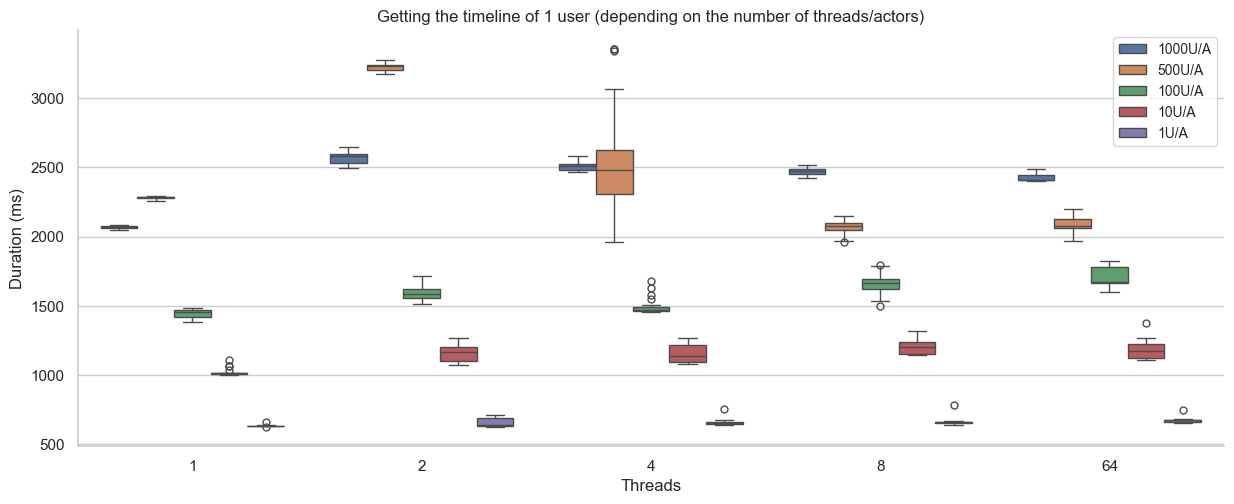
\includegraphics[width = \linewidth]{Images/Speedup(U:A)Box.png}
	\caption{}
\end{figure}
\begin{figure}[H]
	\centering
	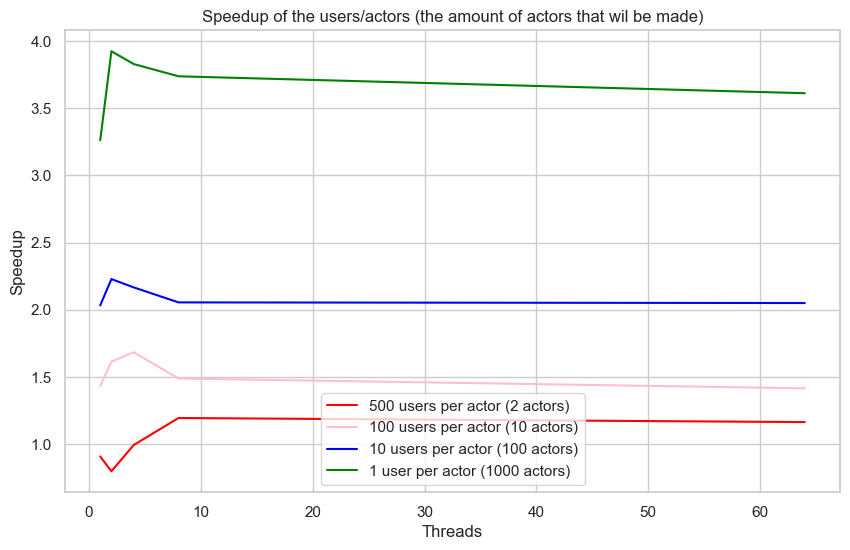
\includegraphics[width = \linewidth]{Images/Speedup(U:A).png}
	\caption{}
\end{figure}
\begin{figure}[H]
	\centering
	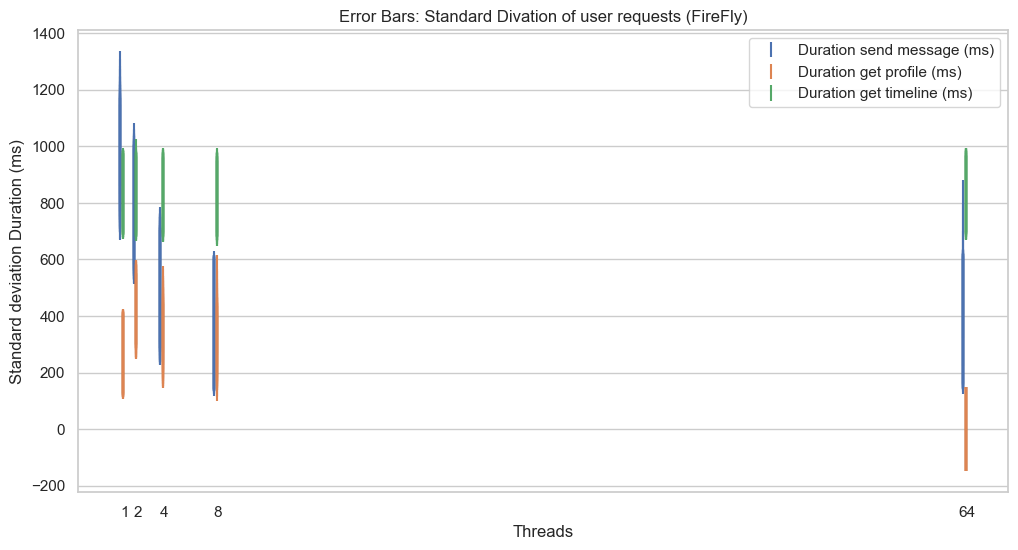
\includegraphics[width = \linewidth]{Images/SpeedupStdURFirefly.png}
	\caption{}
\end{figure}
\begin{figure}[H]
	\centering
	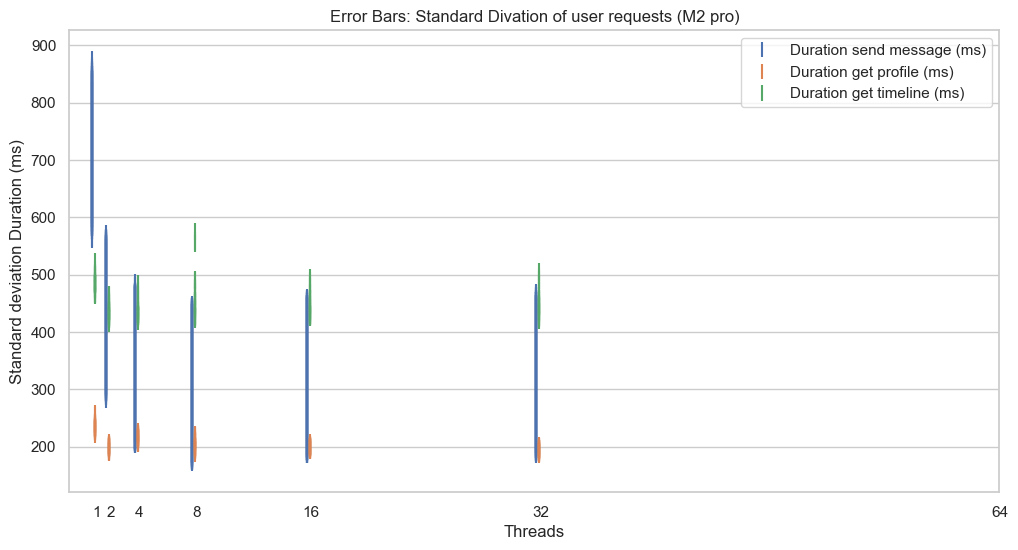
\includegraphics[width = \linewidth]{Images/SpeedupStdUR.png}
	\caption{}
\end{figure}
\begin{figure}[H]
	\centering
	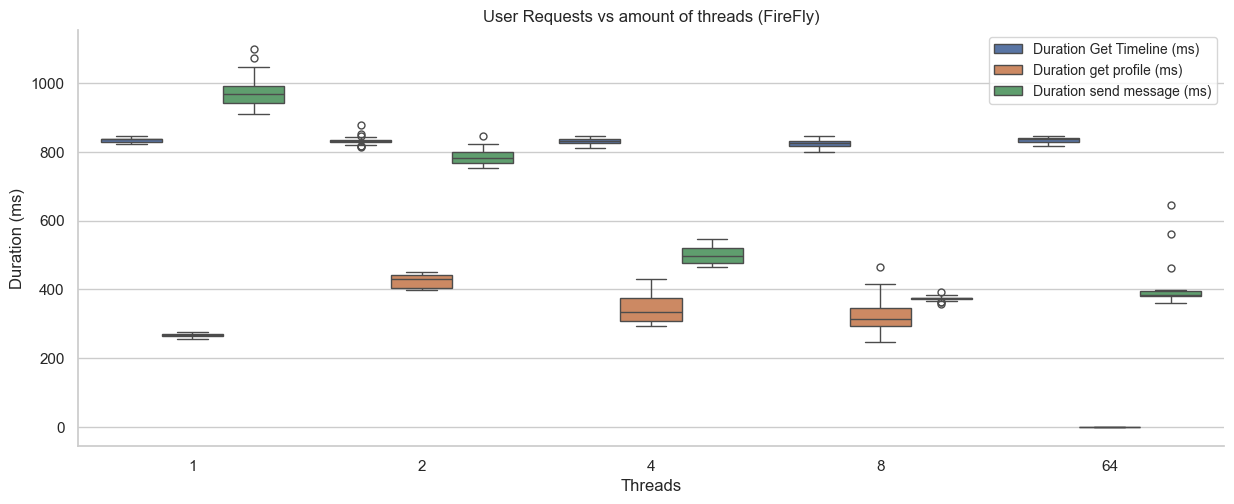
\includegraphics[width = \linewidth]{Images/SpeedupURBoxFirefly.png}
	\caption{}
\end{figure}
\begin{figure}[H]
	\centering
	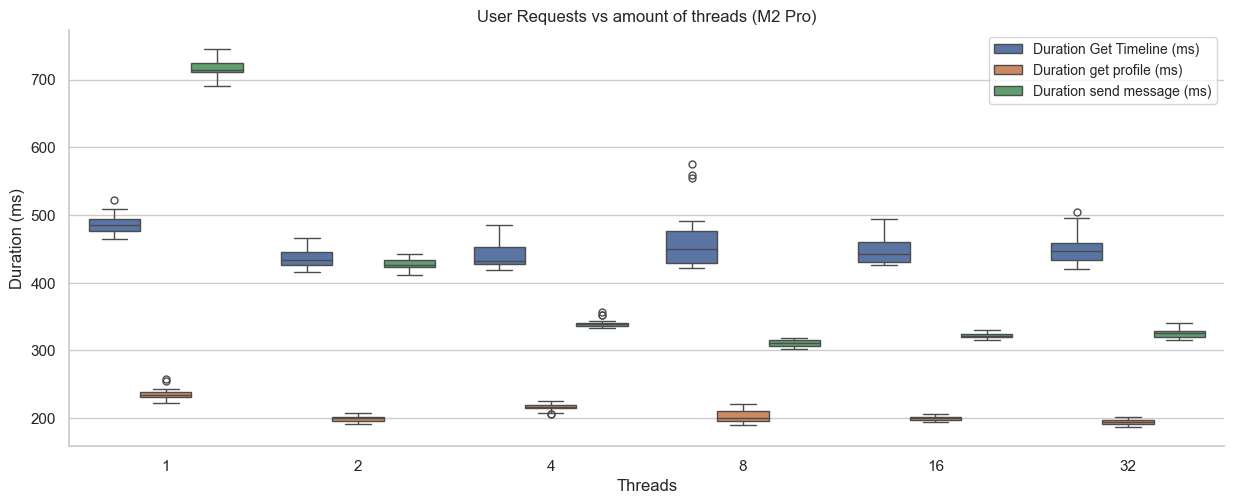
\includegraphics[width = \linewidth]{Images/SpeedupURBox.png}
	\caption{}
\end{figure}
\begin{figure}[H]
	\centering
	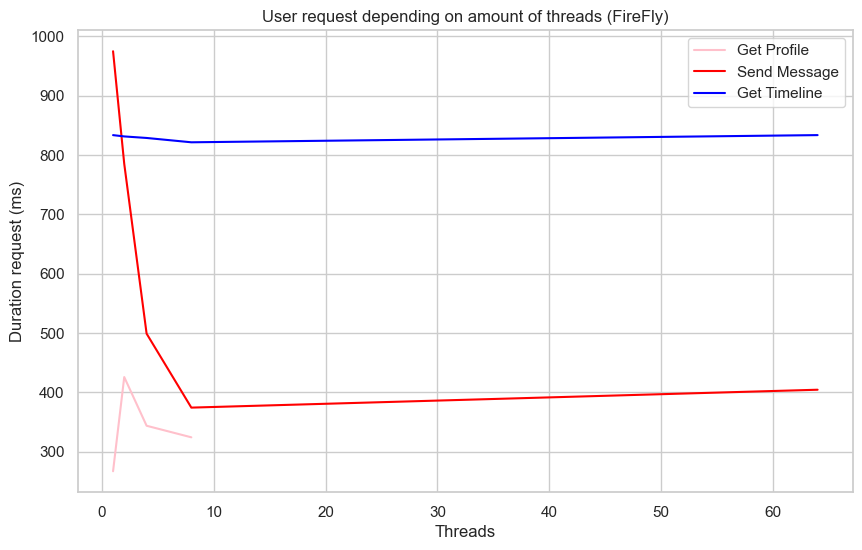
\includegraphics[width = \linewidth]{Images/SpeedupURMeanFirefly.png}
	\caption{}
\end{figure}
\begin{figure}[H]
	\centering
	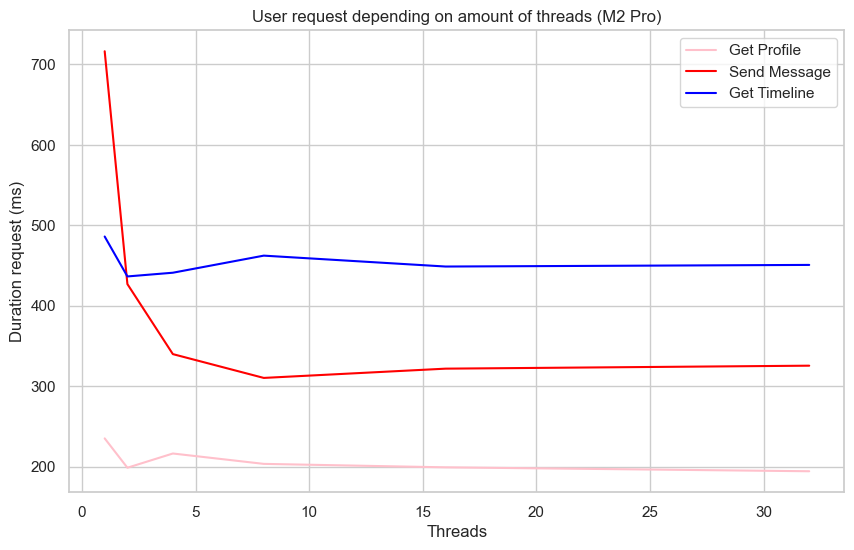
\includegraphics[width = \linewidth]{Images/SpeedupURMean.png}
	\caption{}
\end{figure}
\begin{figure}[H]
	\centering
	\includegraphics[width = \linewidth]{Images/SpeedupURMeanFireflyCom.png}
	\caption{}
\end{figure}
\begin{figure}[H]
	\centering
	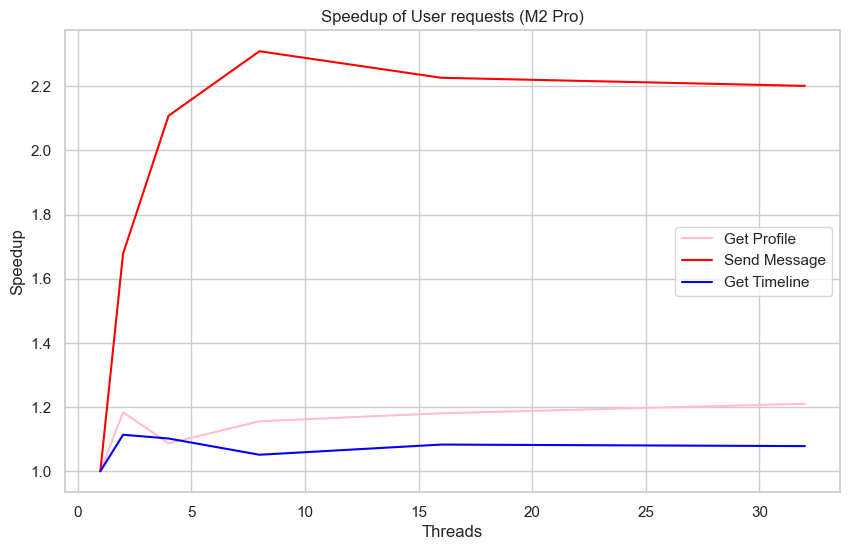
\includegraphics[width = \linewidth]{Images/SpeedupURMeanCom.png}
	\caption{}
\end{figure}

\subsubsection{Results Experiment 2}
\begin{figure}[H]
	\centering
	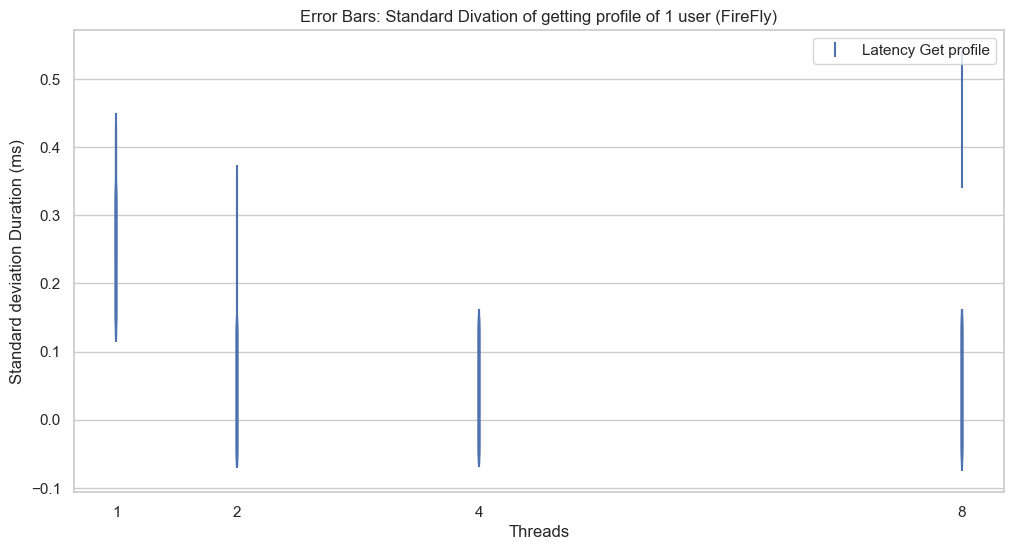
\includegraphics[width = \linewidth]{Images/LatencyStdFirefly.png}
	\caption{}
\end{figure}
\begin{figure}[H]
	\centering
	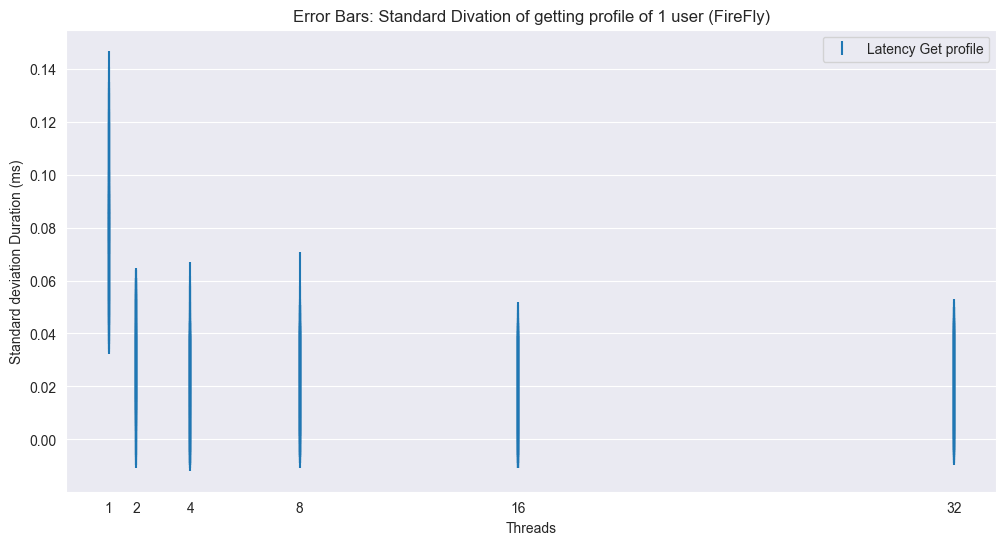
\includegraphics[width = \linewidth]{Images/LatencyStd.png}
	\caption{}
\end{figure}
\begin{figure}[H]
	\centering
	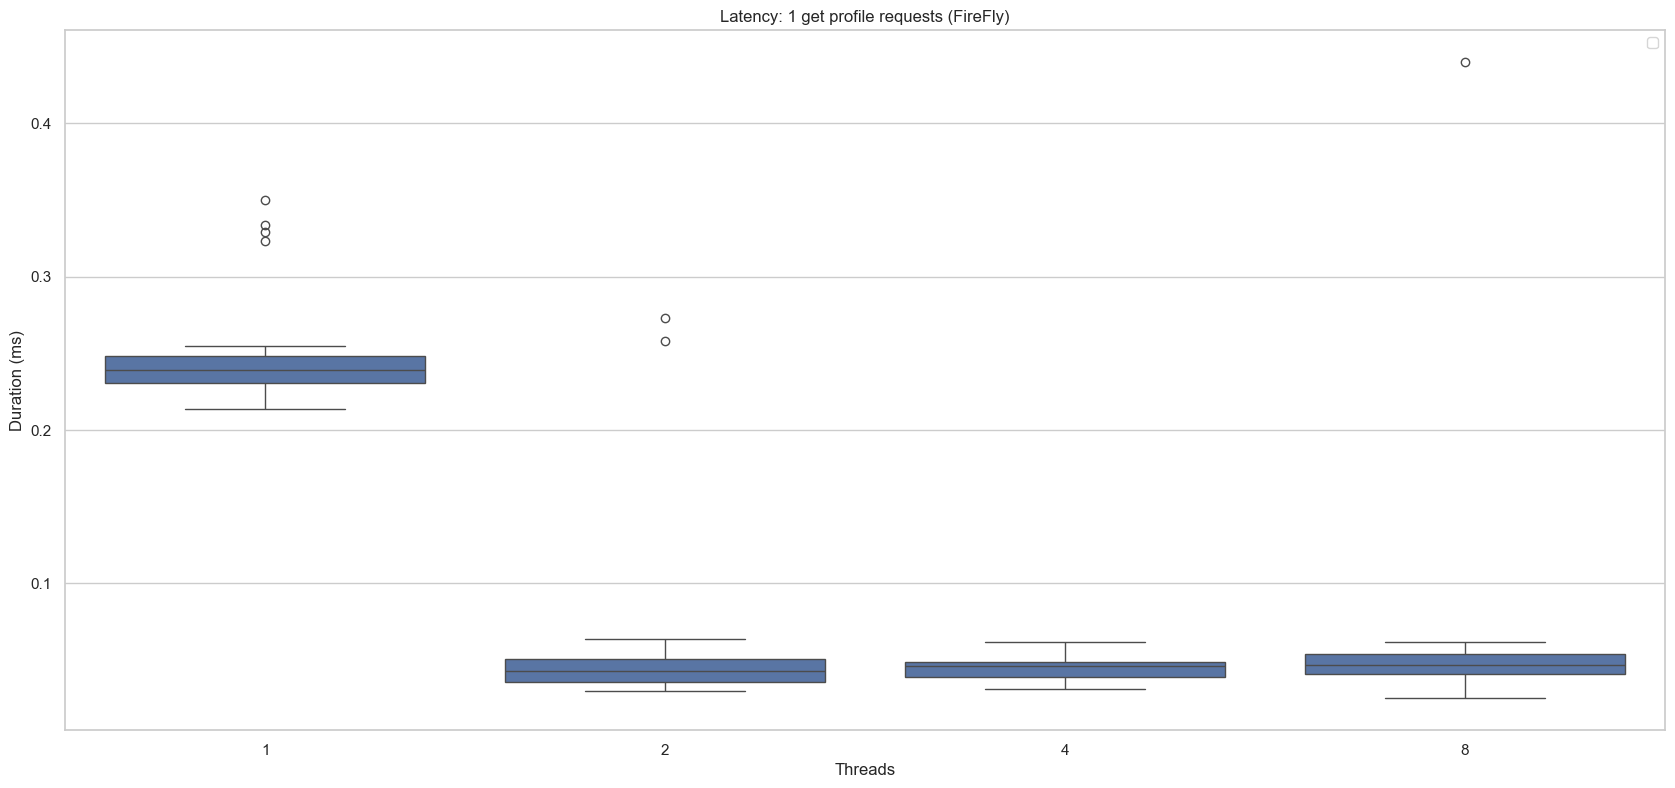
\includegraphics[width = \linewidth]{Images/LatencyBoxFirefly.png}
	\caption{}
\end{figure}
\begin{figure}[H]
	\centering
	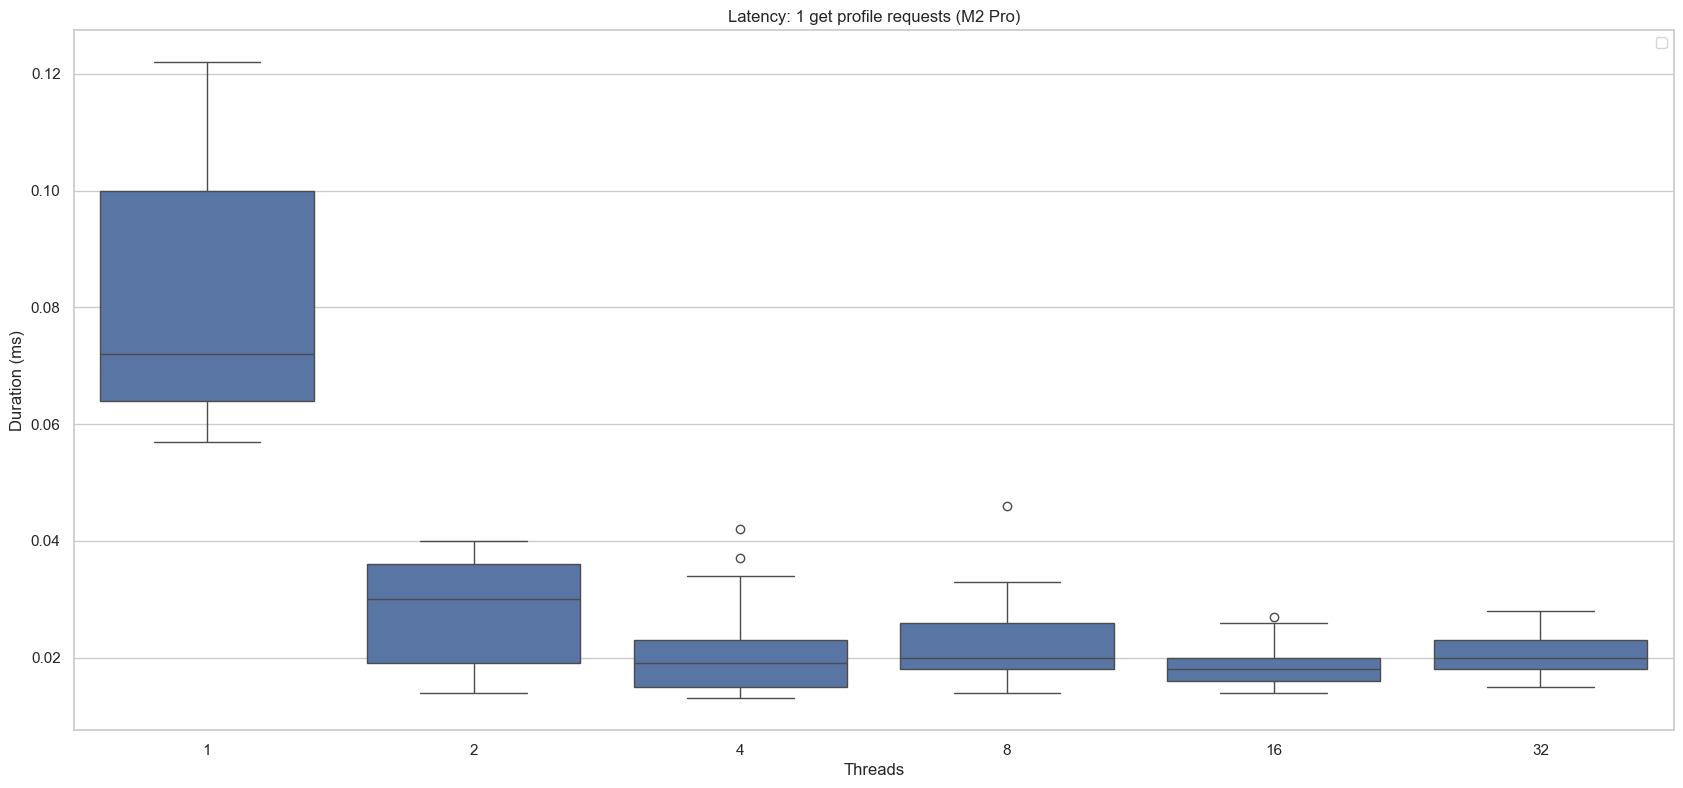
\includegraphics[width = \linewidth]{Images/LatencyBox.png}
	\caption{}
\end{figure}
\begin{figure}[H]
	\centering
	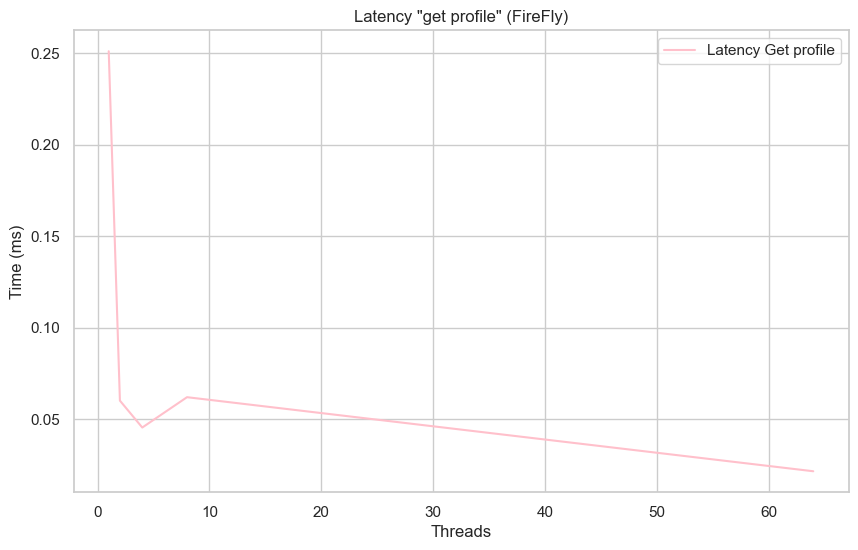
\includegraphics[width = \linewidth]{Images/LatencyProfileFirefly.png}
	\caption{}
\end{figure}
\begin{figure}[H]
	\centering
	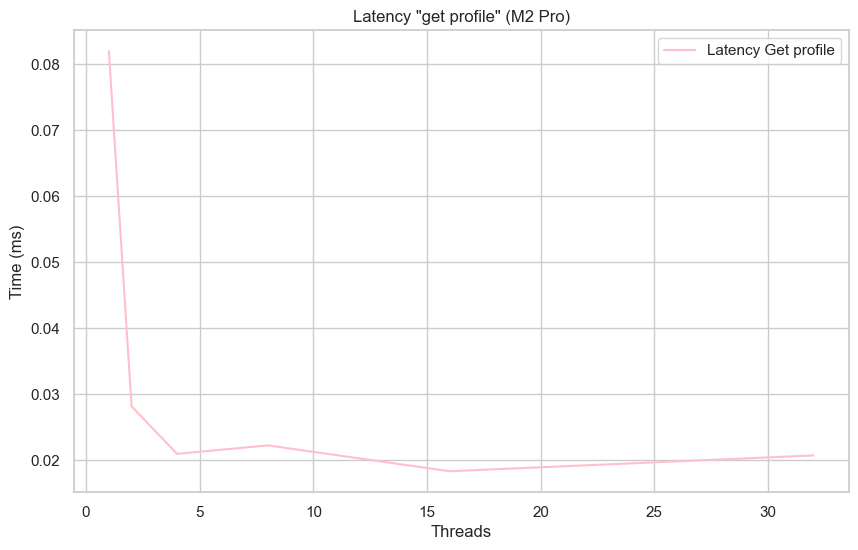
\includegraphics[width = \linewidth]{Images/LatencyProfile.png}
	\caption{}
\end{figure}
\begin{figure}[H]
	\centering
	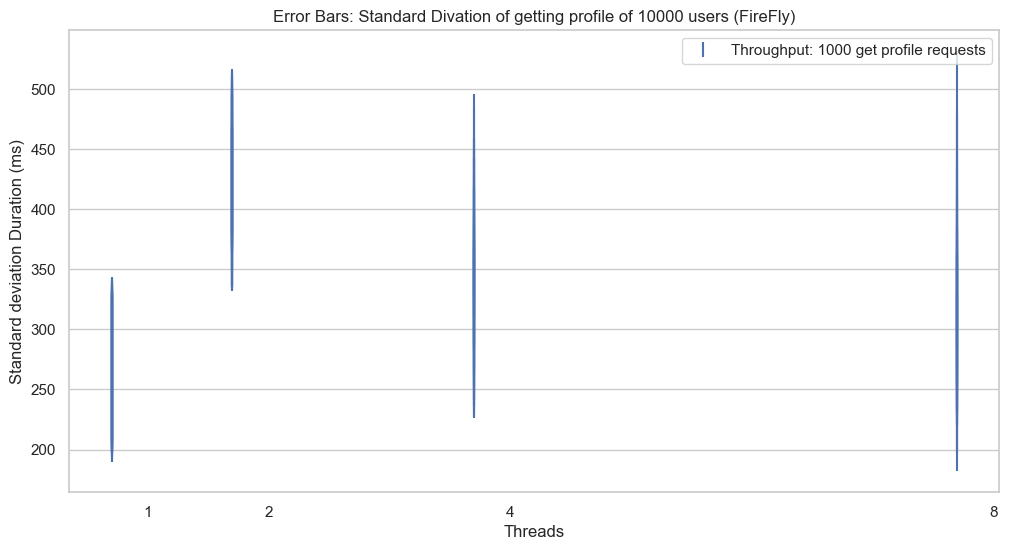
\includegraphics[width = \linewidth]{Images/ThroughputStdFirefly.png}
	\caption{}
\end{figure}

\begin{figure}[H]
	\centering
	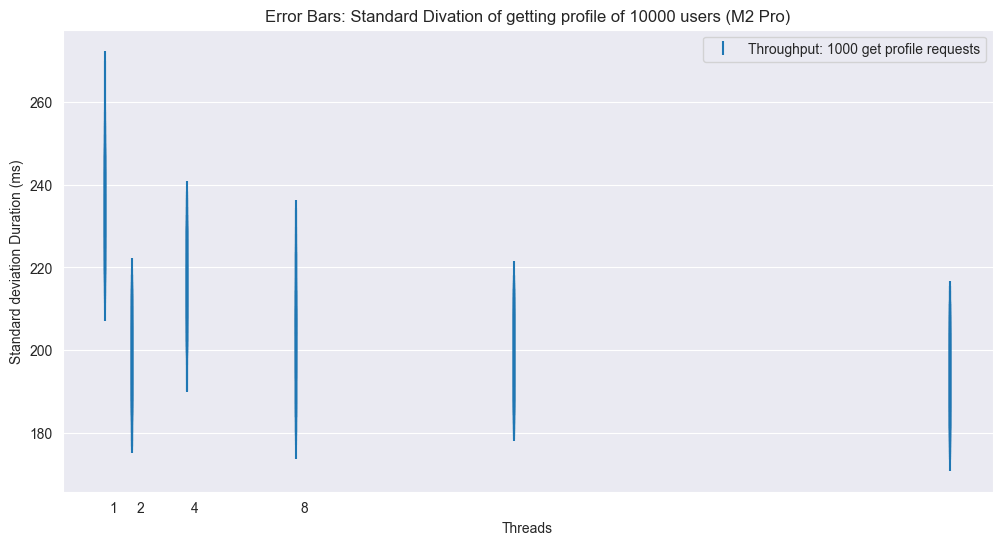
\includegraphics[width = \linewidth]{Images/ThroughputStd.png}
	\caption{}
\end{figure}

\begin{figure}[H]
	\centering
	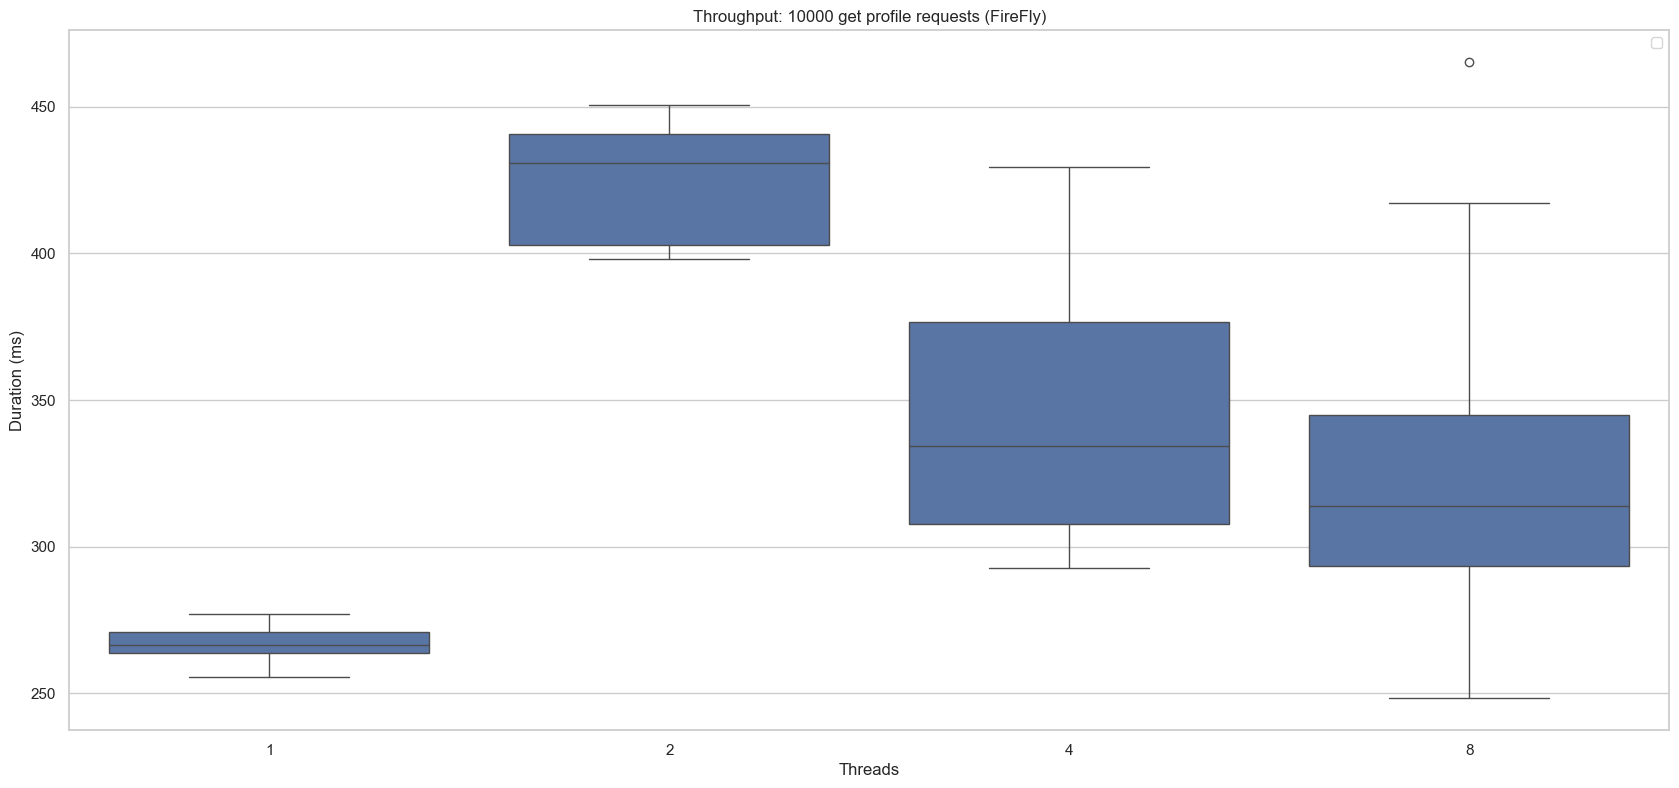
\includegraphics[width = \linewidth]{Images/ThroughputBoxFirefly.png}
	\caption{}
\end{figure}
\begin{figure}[H]
	\centering
	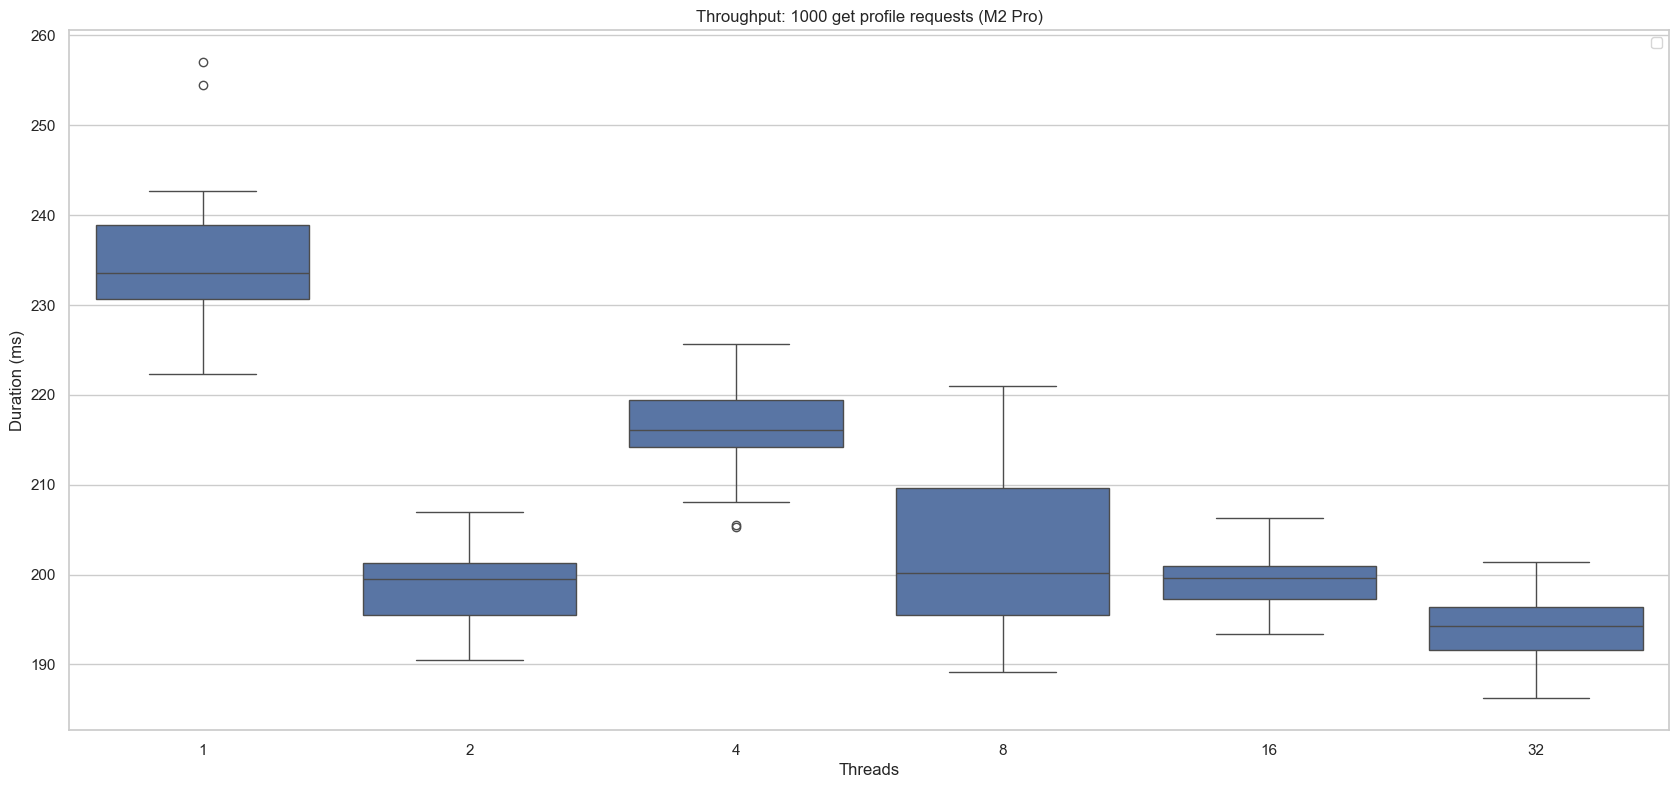
\includegraphics[width = \linewidth]{Images/ThroughputBox.png}
	\caption{}
\end{figure}

\begin{figure}[H]
	\centering
	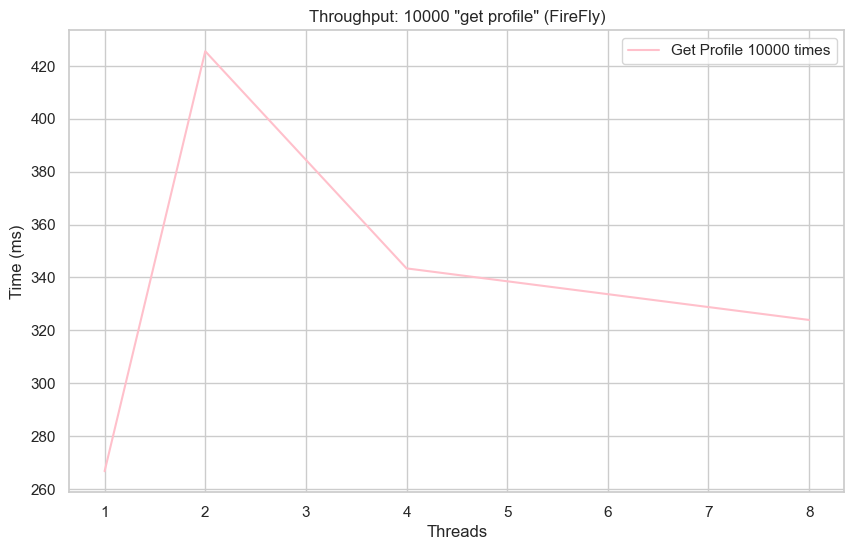
\includegraphics[width = \linewidth]{Images/ThroughputPtofileFirefly.png}
	\caption{}
\end{figure}
\begin{figure}[H]
	\centering
	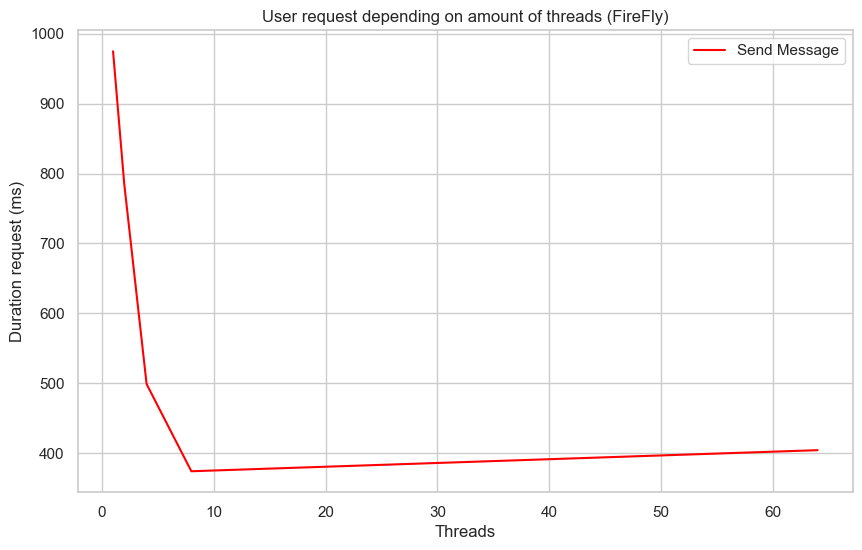
\includegraphics[width = \linewidth]{Images/ThroughputMessageFirefly.png}
	\caption{}
\end{figure}
\begin{figure}[H]
	\centering
	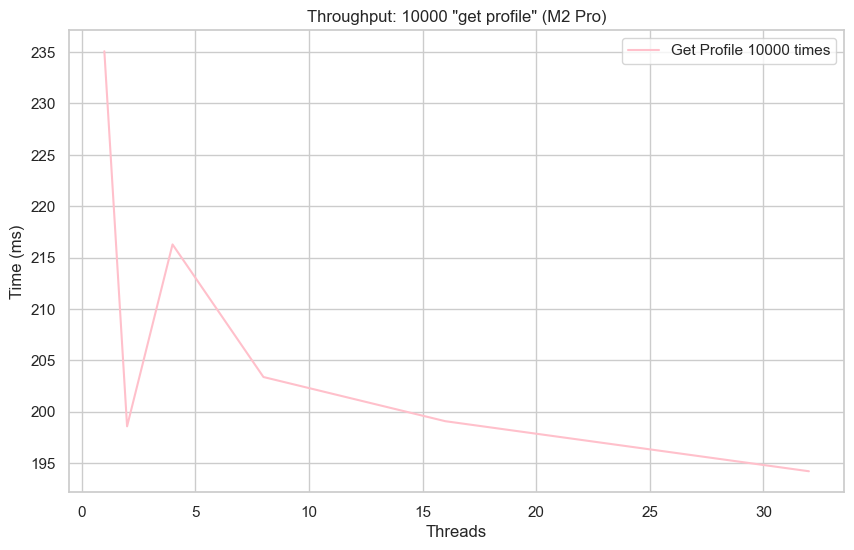
\includegraphics[width = \linewidth]{Images/ThroughputProfile.png}
	\caption{}
\end{figure}
\begin{figure}[H]
	\centering
	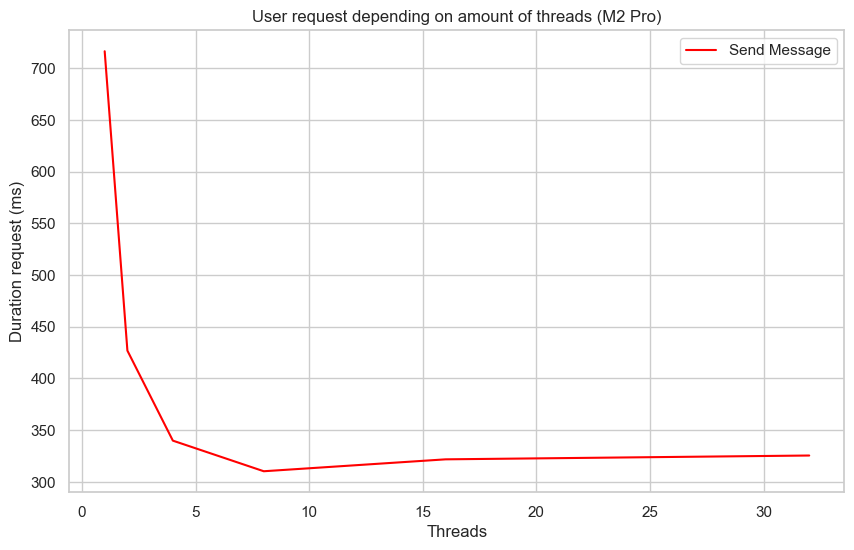
\includegraphics[width = \linewidth]{Images/ThroughputMessage.png}
	\caption{}
\end{figure}

\subsubsection{Results Experiment 3}
\begin{figure}[H]
	\centering
	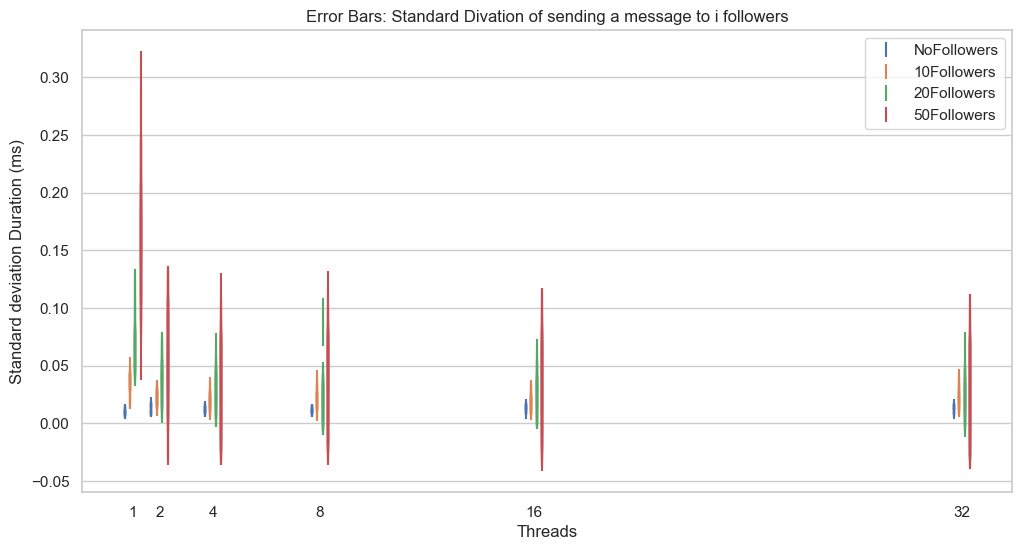
\includegraphics[width = \linewidth]{Images/ErrorBarsLatency.png}
	\caption{}
\end{figure}
\begin{figure}[H]
	\centering
	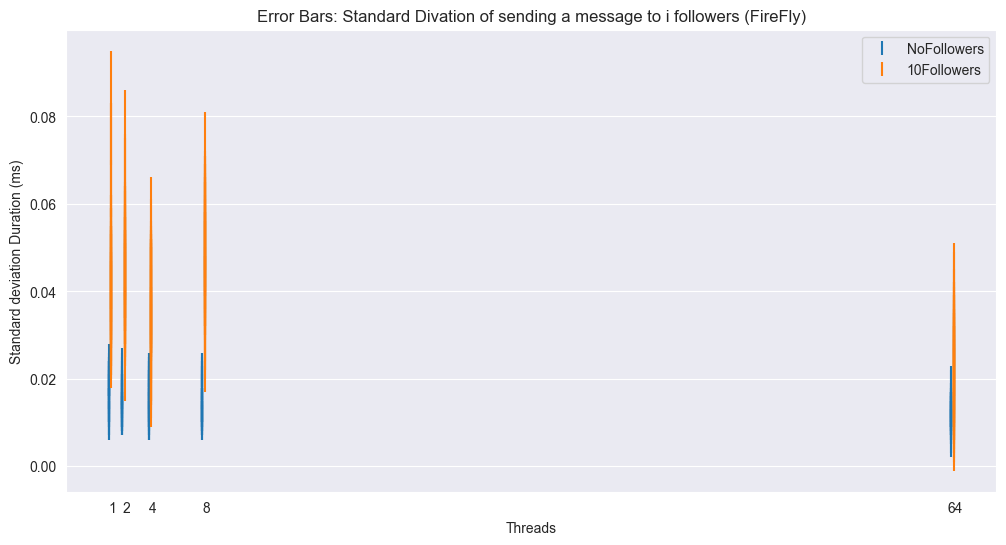
\includegraphics[width = \linewidth]{Images/ErrorBarsLatencyFireFly.png}
	\caption{}
\end{figure}
\begin{figure}[H]
	\centering
	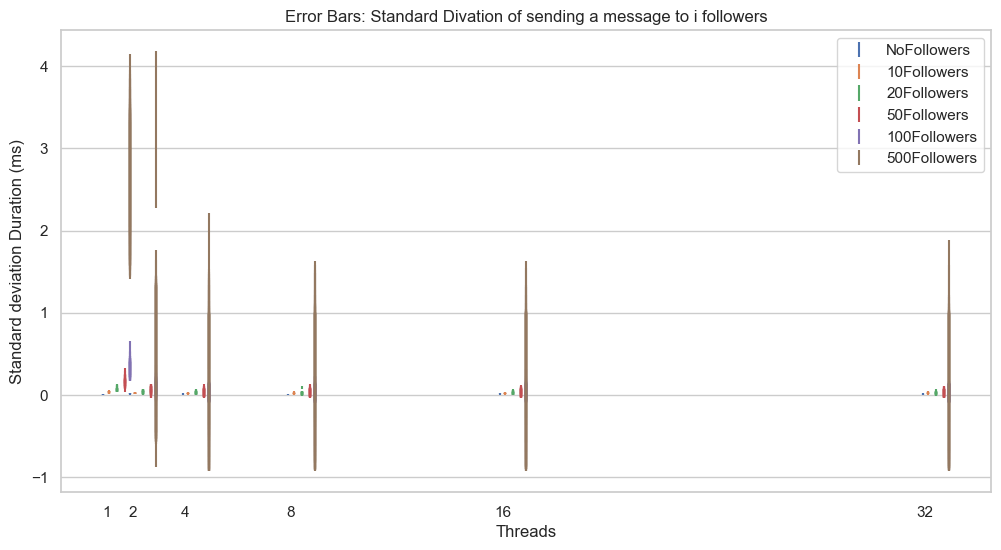
\includegraphics[width = \linewidth]{Images/ErrorBarsLatencyFull.png}
	\caption{}
\end{figure}

\begin{figure}[H]
	\centering
	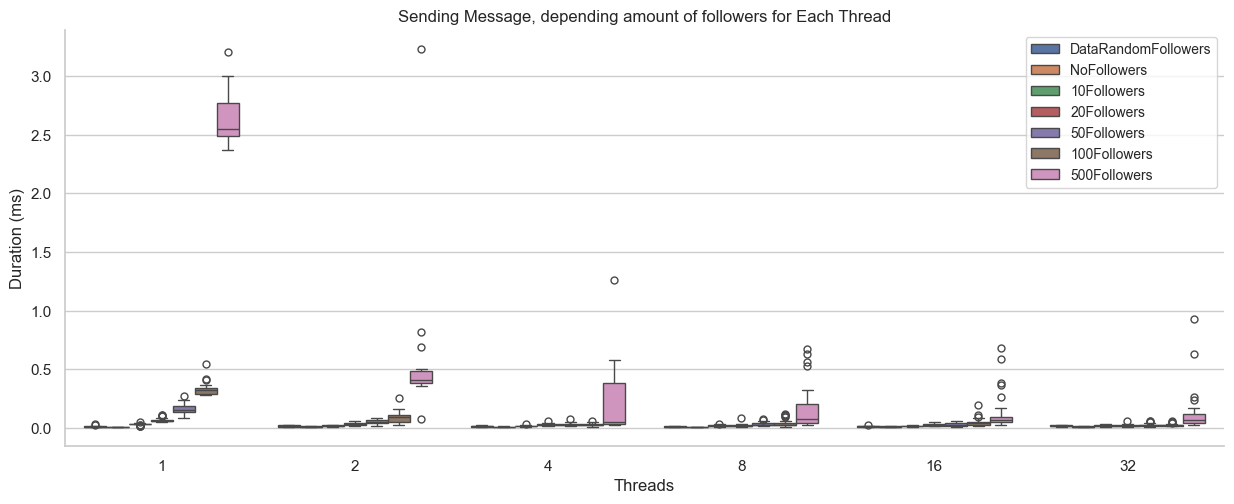
\includegraphics[width = \linewidth]{Images/SendingMessageLatencyBox.png}
	\caption{}
\end{figure}
\begin{figure}[H]
	\centering
	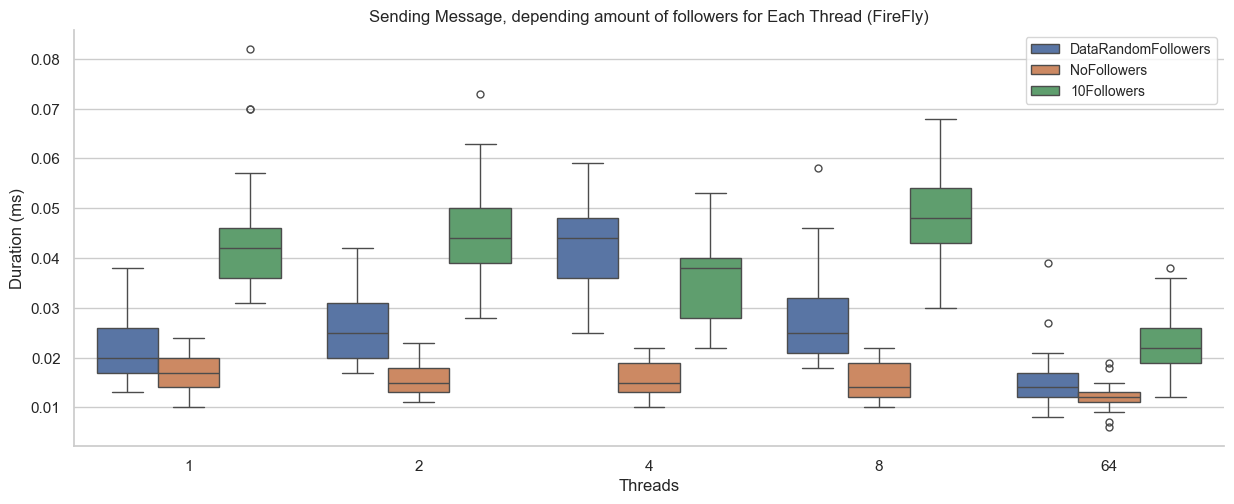
\includegraphics[width = \linewidth]{Images/SendingMessageLatencyBoxFireFly.png}
	\caption{}
\end{figure}

\begin{figure}[H]
	\centering
	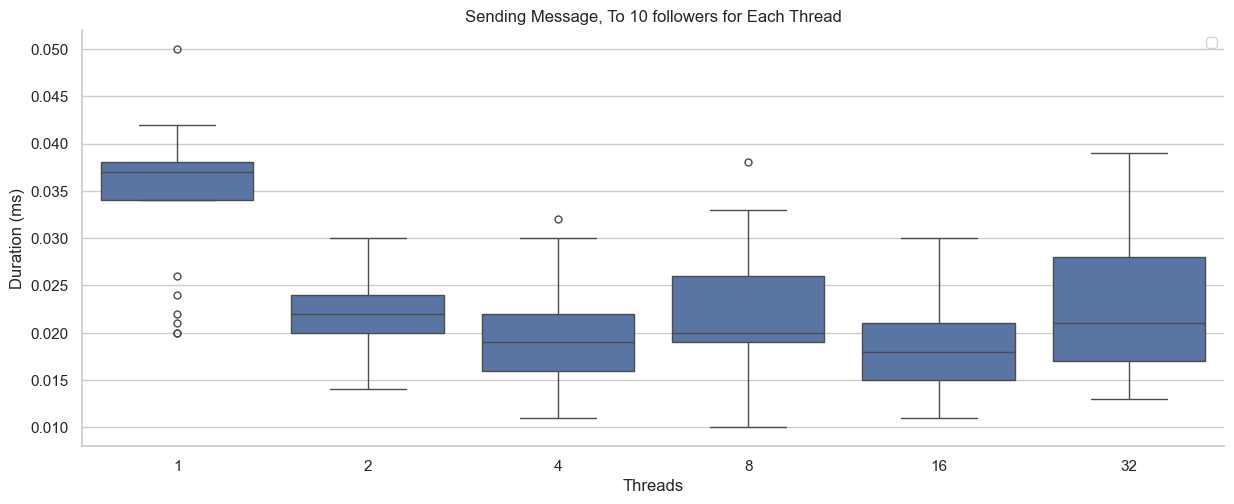
\includegraphics[width = \linewidth]{Images/SendingMessageBox10Follower.png}
	\caption{}
\end{figure}

\begin{figure}[H]
	\centering
	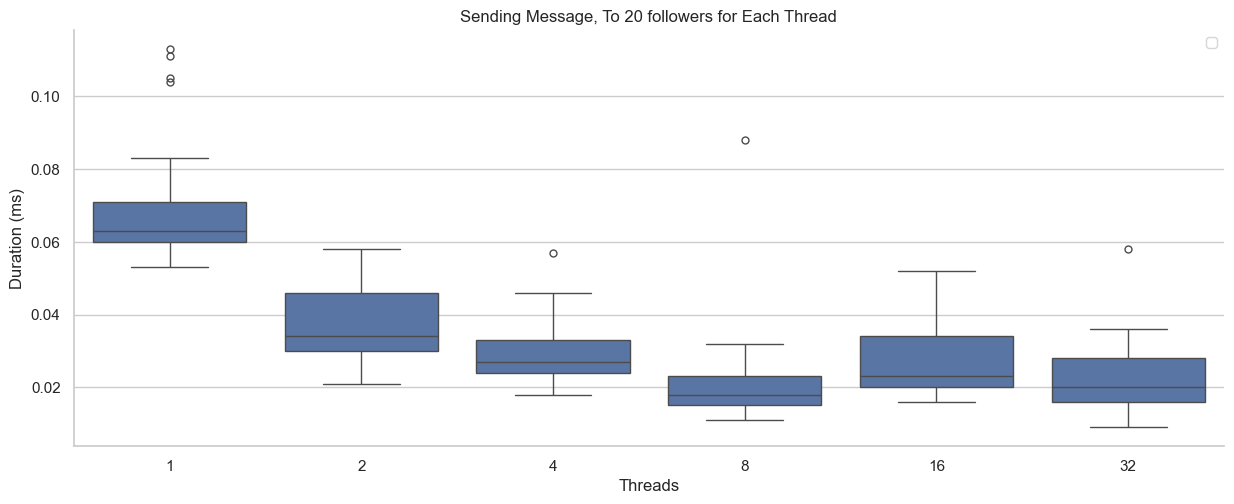
\includegraphics[width = \linewidth]{Images/SendingMessageBox20Follower.png}
	\caption{}
\end{figure}

\begin{figure}[H]
	\centering
	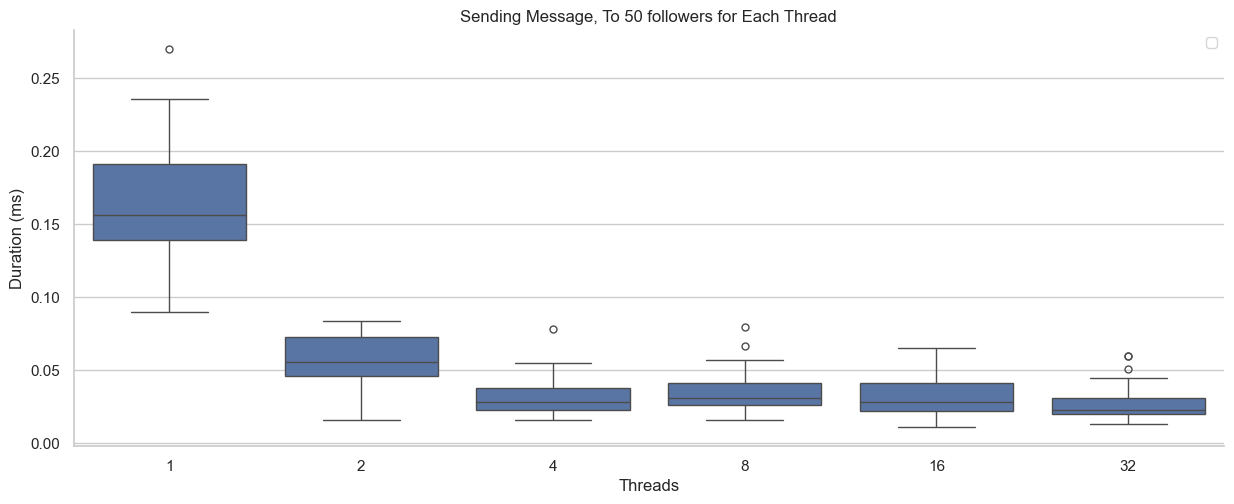
\includegraphics[width = \linewidth]{Images/SendingMessageBox50Followers.png}
	\caption{}
\end{figure}
\begin{figure}[H]
	\centering
	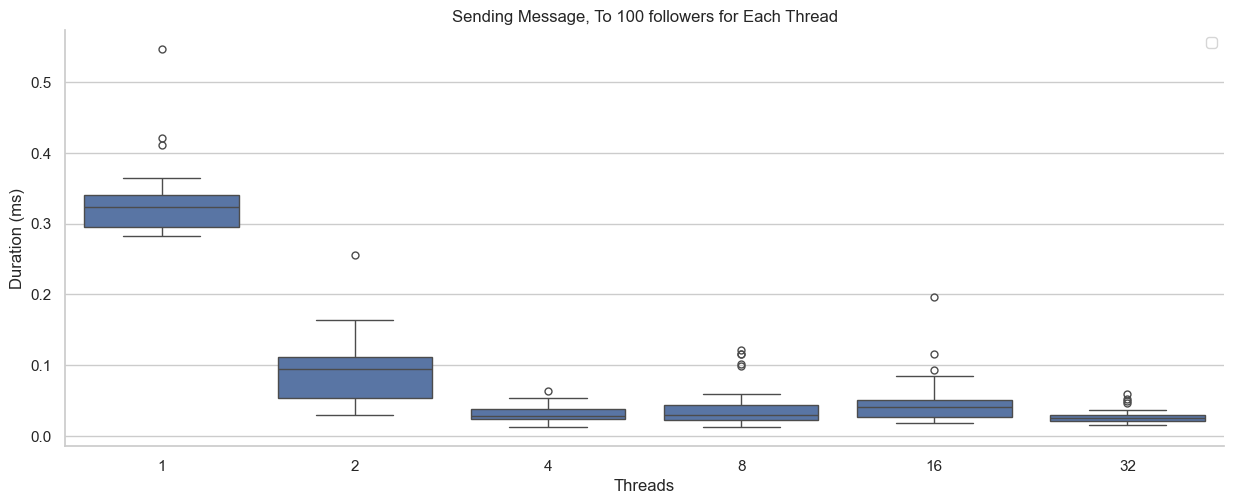
\includegraphics[width = \linewidth]{Images/SendingMessageBox100Follower.png}
	\caption{}
\end{figure}
\begin{figure}[H]
	\centering
	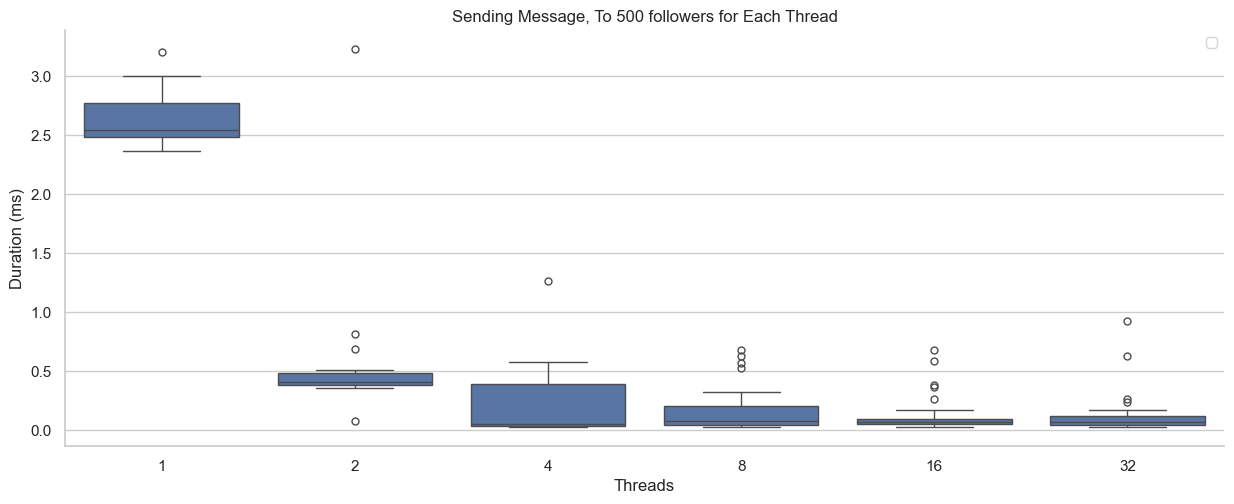
\includegraphics[width = \linewidth]{Images/SendingMessageBox500Follower.png}
	\caption{}
\end{figure}

\begin{figure}[H]
	\centering
	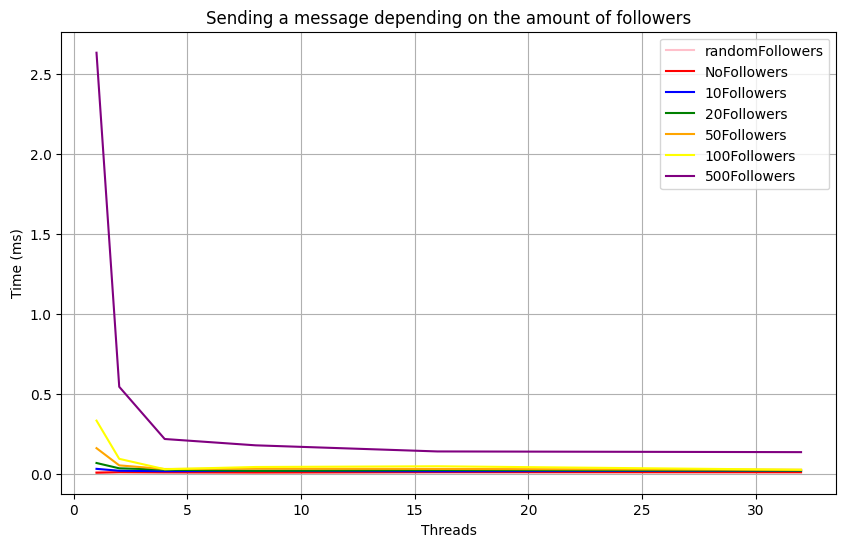
\includegraphics[width = \linewidth]{Images/SendingMessageLatencyMean.png}
	\caption{}
\end{figure}
\begin{figure}[H]
	\centering
	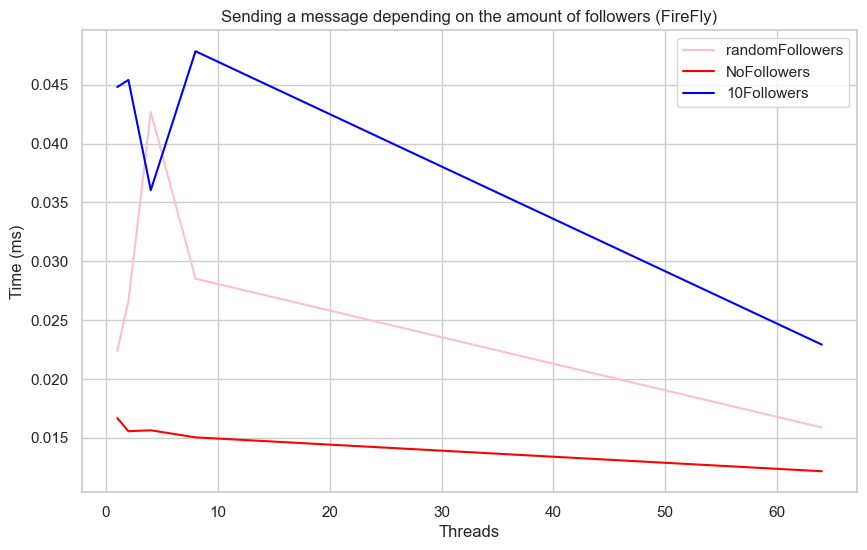
\includegraphics[width = \linewidth]{Images/SendingMessageLatencyMeanFireFly.png}
	\caption{}
\end{figure}

\begin{figure}[H]
	\centering
	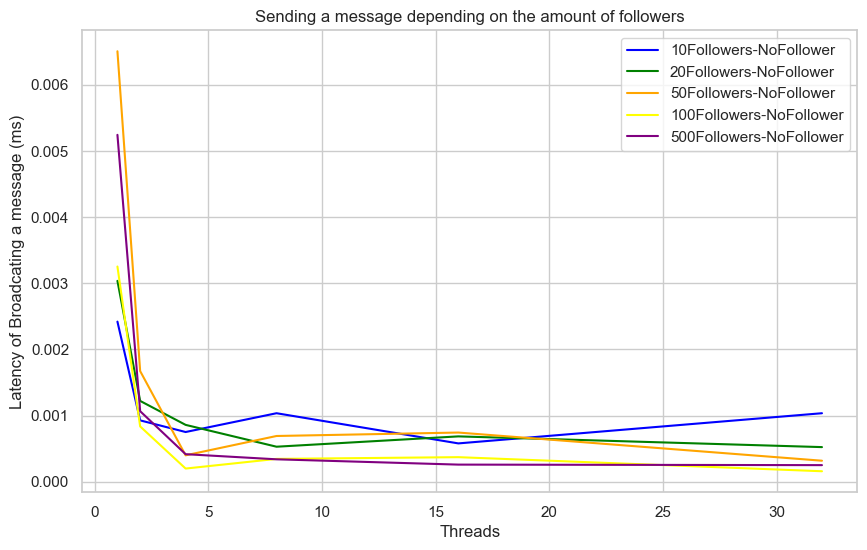
\includegraphics[width = \linewidth]{Images/SendingMessageLatency-Mean.png}
	\caption{}
\end{figure}



\subsubsection{ Report results appropriately: use diagrams, report averages or medians and measurement
errors, possibly use box plots. Graphical representations are preferred over large tables
with many numbers. Describe what we see in the graph in your report text.}


\subsubsection{Interpret the results: explain why we see the results we see. Relate the results back to
your architecture: how did your design decisions influence these results? If the results
contradict your intuition, explain what caused this.}

\section{Insight Question}
Briefly answer the questions below (max. 250 words, or ~2 paragraphs, each):

\begin{itemize}
	\item spawning a process in Erlang is a very lightweight operation: a newly spawned Erlang process only uses 309 words of memory. How has this influenced your solution? Imagine the cost of
creating a process was much higher, e.g. if you were using Java and created new Threads: how
would this affect the performance and how could you improve this?
	\item  Twitter and Threads provide two types of homepage: "Following" and "For You". 
		The page "Following" contains the timeline as we implemented it, consisting of a chronological list of
messages from the users you follow. The page "For You" contains a list of messages that are
gathered both from users you follow as well as other "popular" messages on the platform,
and are then sorted using a machine learning algorithm. How would you implement this in
your system? Do not focus on the machine learning algorithm, but discuss the impact on the
architecture and performance of your system.

\end{itemize}

%\bibliography{bibliography}
\end{document}
